\chapter{Metodologia}

%%%%%%%%%%%%%%%%%%%%%%%%%%%%%%%%%%%
\section{Sistemas de Controle}

\subsection{Modelo Motor DC}
\begin{figure}[H]
  \caption{Modelo do Motor DC}
  \begin{center}
      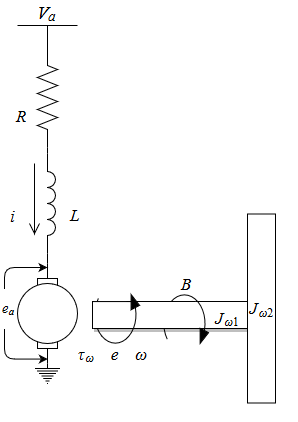
\includegraphics[scale=.8]{img/modelo_motor_dc}
  \end{center}
  \fonte{Elaborado pelo Autor.} 
  \label{fig:modelo_motor_dc}
\end{figure}

\subsection{Modelo Completo do Satélite}

\begin{figure}[H]
  \caption{Modelo em malha aberta}
  \begin{center}
      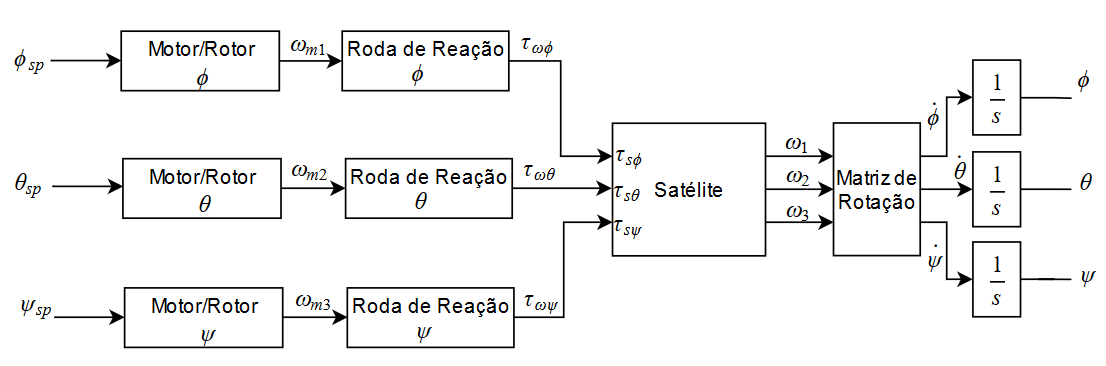
\includegraphics[scale=.55]{img/modelo_satelite_malha_aberta}
  \end{center}
  \fonte{Elaborado pelo Autor.} 
  \label{fig:modelo_satelite_malha_aberta}
\end{figure}


\begin{figure}[H]
  \caption{Modelo em malha fechada e com um Controlador PID}
  \begin{center}
      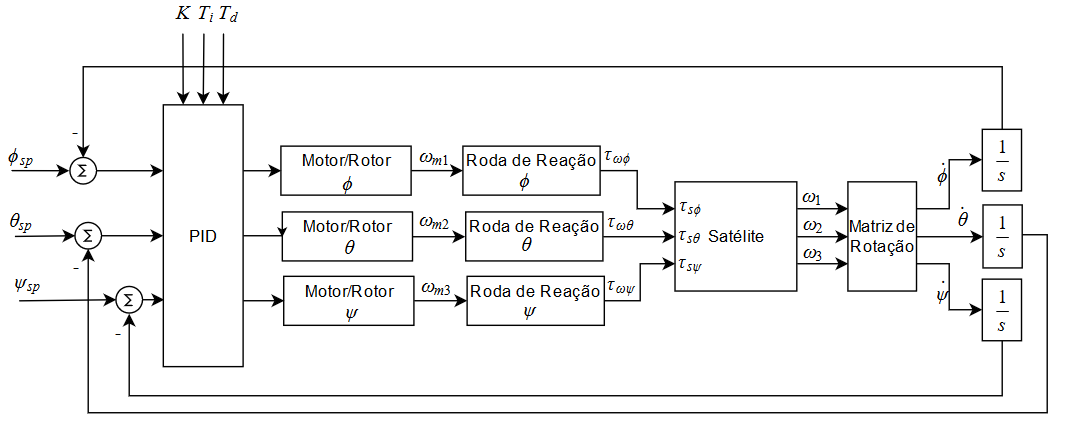
\includegraphics[scale=.55]{img/modelo_satelite_pid}
  \end{center}
  \fonte{Elaborado pelo Autor.} 
  \label{fig:modelo_satelite_pid}
\end{figure}


%%%%%%%%%%%%%%%%%%%%%%%%%%%%%%%%%%%%%%%%%%%%%%%%%%%%%%%%%%%%%%%%%%%%%%
\section{Software}

\begin{figure}[H]
  \caption{Topologia de Rede}
  \begin{center}
      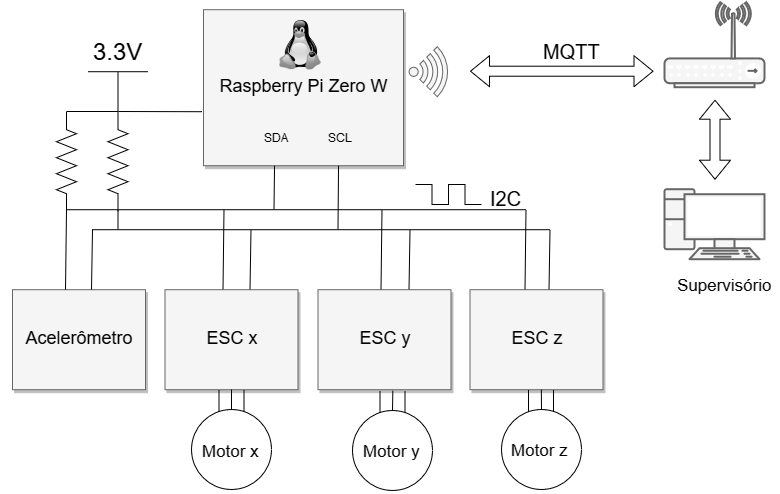
\includegraphics[scale=.75]{img/comunicacao_projeto}
  \end{center}
  \fonte{Elaborado pelo Autor.} 
  \label{fig:comunicacao_projeto}
\end{figure}

%%%%%%%%%%%%%%%%%%%%%%%%%%%%%%%%%%%
\subsection{Implementação do Controlador PID}

%%%%%%%%%%%%%%%%%%%%%%%%%%%%%%%%%%%
\subsection{Implementação da Rede Neural}

%%%%%%%%%%%%%%%%%%%%%%%%%%%%%%%%%%%
\subsection{Protocolos de Comunicação}

%%%%%%%%%%%%%%%%%%%%%%%%%%%%%%%%%%%
\subsection{Sistemas Supervisórios}


%%%%%%%%%%%%%%%%%%%%%%%%%%%%%%%%%%%%%%%%%%%%%%%%%%%%%%%%%%%%%%%%%%%%%%
\section{Hardware}


%%%%%%%%%%%%%%%%%%%%%%%%%%%%%%%%%%%
\subsection{Modelagem Motor DC e Rodas de Reação}

\begin{figure}[H]
  \caption{Desenho mecânico do conjunto Motor-Roda}
  \begin{center}
      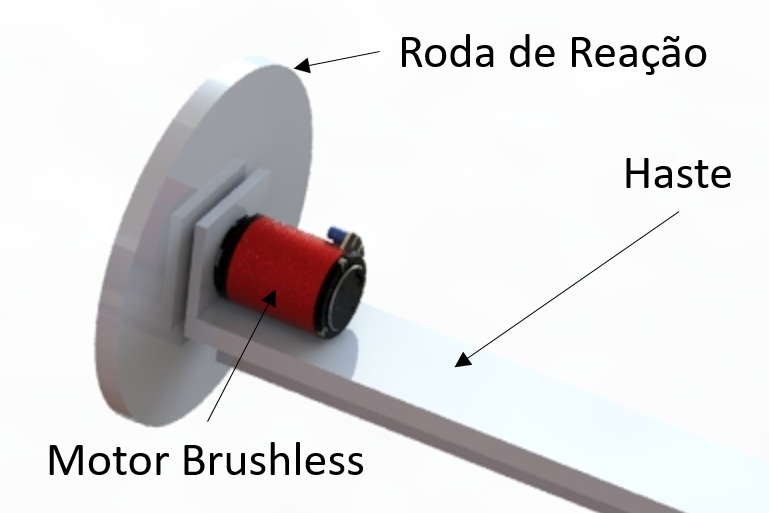
\includegraphics[scale=.45]{img/motor_roda_desenho}
  \end{center}
  \fonte{Elaborado pelo Autor.} 
  \label{fig:motor_roda_desenho}
\end{figure}


%%%%%%%%%%%%%%%%%%%%%%%%%%%%%%%%%%%
\subsection{Mancal a Ar}

\begin{figure}[H]
  \caption{Desenho Mecânico do Mancal a Ar}
  \begin{center}
      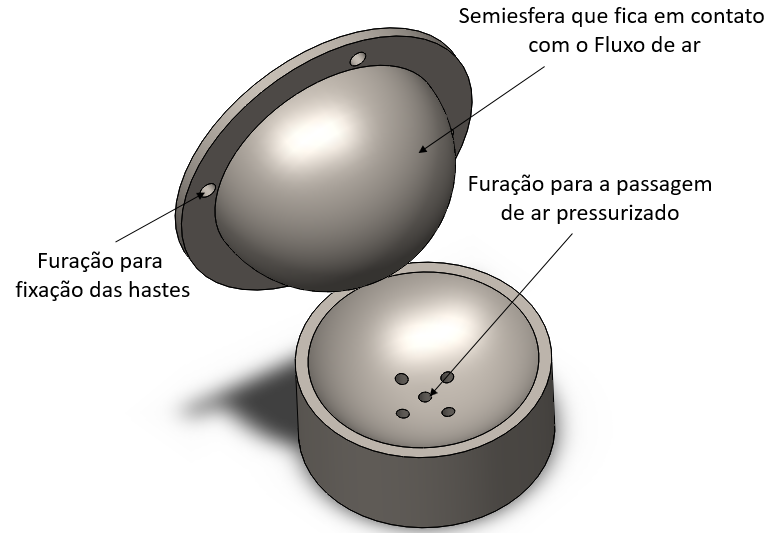
\includegraphics[scale=.45]{img/base_desenho}
  \end{center}
  \fonte{Elaborado pelo Autor.} 
  \label{fig:base_desenho}
\end{figure}


%%%%%%%%%%%%%%%%%%%%%%%%%%%%%%%%%%%
\subsection{Corpo do Simulador de Satélites}

\begin{figure}[H]
  \caption{Desenho Mecânico do Satélite Completo}
  \begin{center}
      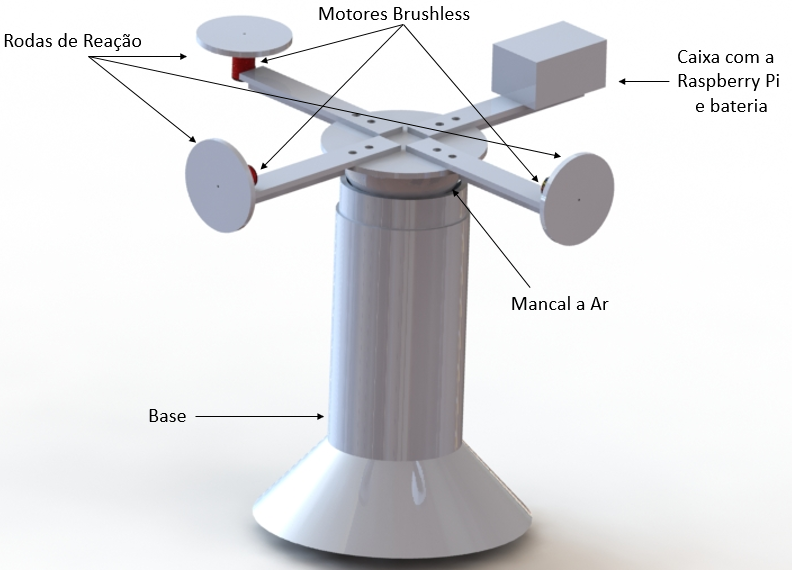
\includegraphics[scale=.75]{img/satelite_completo}
  \end{center}
  \fonte{Elaborado pelo Autor.} 
  \label{fig:satelite_completo}
\end{figure}

%%%%%%%%%%%%%%%%%%%%%%%%%%%%%%%%%%%
\subsection{Elementos Eletrônicos}

\begin{figure}[H]
  \caption{Raspberry Pi Zero}
  \begin{center}
      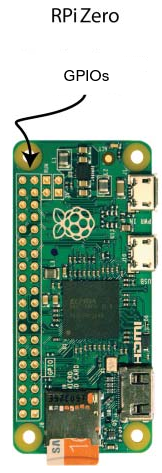
\includegraphics[scale=.55]{img/rasp_zero}
  \end{center}
  \fonte{Adaptado de \citeonline{Molloy2016}} 
  \label{fig:rasp_zero}
\end{figure}


\begin{figure}[H]
  \caption{Circuito impresso com o acelerômetro MMA7260QT}
  \begin{center}
      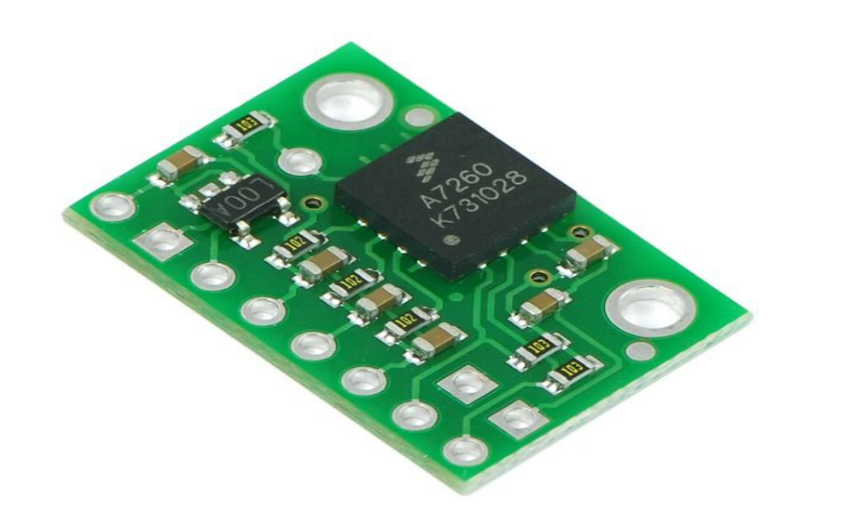
\includegraphics[scale=.45]{img/pci_acelerometro_calache_p22}
  \end{center}
  \fonte{Calache, Danilo Carreiro} 
  \label{fig:pci_acelerometro_calache_p22}
\end{figure}
